\documentclass[]{article}


% included packages
% used to include images
\usepackage{graphicx}
% used to add caption to figures, tables, etc.
\usepackage{caption}
% used to add captions to subfigures
\usepackage{subcaption}
% make tables span over more than one page
\usepackage{longtable}
% to avoid the use of static table widths
\usepackage{tabularx}
% add hyperlinks in the texts
\usepackage{hyperref}

% correct bad hyphenation here
\hyphenation{}

% remove heading of bibliography as it is located in a subsection with text
\makeatletter
\renewenvironment{thebibliography}[1]{%
%     \section*{\refname}%
%      \@mkboth{\MakeUppercase\refname}{\MakeUppercase\refname}%
      \list{\@biblabel{\@arabic\c@enumiv}}%
           {\settowidth\labelwidth{\@biblabel{#1}}%
            \leftmargin\labelwidth
            \advance\leftmargin\labelsep
            \@openbib@code
            \usecounter{enumiv}%
            \let\p@enumiv\@empty
            \renewcommand\theenumiv{\@arabic\c@enumiv}}%
      \sloppy
      \clubpenalty4000
      \@clubpenalty \clubpenalty
      \widowpenalty4000%
      \sfcode`\.\@m}
     {\def\@noitemerr
       {\@latex@warning{Empty `thebibliography' environment}}%
      \endlist}
\makeatother


\begin{document}

% paper title
% can use linebreaks \\ within to get better formatting as desired
\title{Need4Feed: \\
Software Specification\\
by BIT}


% author names and affiliations
% use a multiple column layout for up to three different
% affiliations
\author{Brian Pohl\\
Student ID: 9100920124\\
\texttt{enzothebaker8@gmail.com}
\and
Iker Trun\\
Student ID: 9101920127\\
\texttt{iktrun@gmail.com}
\and
Thomas Ingvarsson\\
Student ID: 9093920122\\
\texttt{ingvarsson.thomas@sillys.se}
}


% make the title area
\maketitle


\section*{Revision History}
\begin{center}
    \begin{tabularx}{\linewidth}{ | l | l | X | l |}
    \hline
    \textbf{Version} & \textbf{Date} & \textbf{Description} & \textbf{Author}\\ \hline
    0.1 & 09-Oct-2012 & First draft. & T. Ingvarsson\\ \hline
    0.11 & 09-Oct-2012 & Added Revision History and Table of Contents. & T. Ingvarsson\\ \hline
    0.12 & 09-Oct-2012 & Detailed Requirements table has been remade into a multi-page table. & T. Ingvarsson\\ \hline
    0.13 & 14-Oct-2012 & Stream-lined the abstract and introduction to not have too much redundancy. & T. Ingvarsson\\ \hline
    0.14 & 15-Oct-2012 & Software Interfaces is rewritten as pure requirements that do not imply how it should be solved. & T. Ingvarsson \\ \hline
    0.15 & 15-Oct-2012 & Major overhaul of User Interfaces. Simplified and removed unnecessary descriptions. To strict requirements are removed at this stage. & T. Ingvarsson\\ \hline
    0.16 & 15-Oct-2012 & Major overhaul of Product Features. Added a use case diagram including a better overview of the features as well as a list of actors to the system. & T. Ingvarsson\\ \hline
    0.17 & 16-Oct-2012 & Simplified the System Features section by removing the functional requirements of every subsection, this will be covered in the detailed requirement list anyway. Removed feed list and all with it, is not a feature requirement.  Removed subsection Manage Categories as this is covered in Manage Feeds. & T. Ingvarsson\\ \hline
    0.18 & 19-Oct-2012 & Added References. & T. Ingvarsson\\ \hline
    0.19 & 23-Oct-2012 & Added Software Quality Attributes to Other Non-functional Requirements. & T. Ingvarsson\\ \hline
    0.20 & 23-Oct-2012 & Updated use case diagram with more sub-features. Updated System Features to match the use case diagram. & T. Ingvarsson\\ \hline
    % copy the last line before adding the new revision.
    \end{tabularx}
    
    % new page of revision history
    \begin{tabularx}{\linewidth}{ | l | l | X | l |}
    \hline
    \textbf{Version} & \textbf{Date} & \textbf{Description} & \textbf{Author}\\ \hline
    0.21 & 24-Oct-2012 & Update the Detailed Requirement list to match the rest of the updates. & T. Ingvarsson\\ \hline
    0.22 & 27-Oct-2012 & Added new features; Share Post, Import Feed(s), Export Feed(s), Find Similar Feed(s). Changed so it should handle multiple kinds of sources, not just RSS. & T. Ingvarsson\\ \hline
    0.30 & 21-Nov-2012 & Added comparison table of the most popular readers existing on the Google Play Store to clarify the differences. & T. Ingvarsson\\ \hline
    0.31 & 26-Nov-2012 & Added a system feature; gather and display statistics. Also updated the deadlines mentioned under project constraints. & T. Ingvarsson\\ \hline
     &  &  & \\ \hline
    % copy the last line before adding the new revision.
    \end{tabularx}
\end{center}


\setcounter{tocdepth}{2}
\tableofcontents


\section{Introduction}


\subsection{Purpose}
The purpose of this document is to specify a software for Android users enabling the functionality to gather, organize and read feeds, regardless of if it is a RSS\cite{rss-spec}, ATOM\cite{atom}, Podcasts or social medium feed. Furthermore, this requirement specification will act as base for the specification which in turn will be the base of the design document. This will be the first release of the mentioned software which is completely standalone in the sense that it is not part of a larger system.


\subsection{Intended Audience and Reading Suggestions}
The intended audience for this document are those with an engineering background interested in this project, whether it be the actual teacher assigning this project to the project group, one of the group members or an actual user wanting to know more about the product or continue development. Due to the small size of the actual product I would recommend all readers to read the whole document from start to finish. However to understand the major features, section~\ref{sec:overall_description} will do. If one is only interested in the actual requirements they are listed in section~\ref{sec:detailed_requirements}, Detailed Requirements. A section in which all requirements are listed with their ID, short description, priority and source.


\subsection{Project Scope}
Nowadays the most common form of communication between people all over the world is taking place on the Internet, or specifically through media such as social networks, forums, and blogs. Blogging has become more and more popular during over the last ten years. The blog is an information sharing tool that allows the user to write about anything that is interesting for him or her and potentially for others with common interests. Through low-maintenance web-based solutions there is also almost no technical knowledge required, compared to more complex web pages, for a user to start and maintain a blog. On the other side taking in information has become just as easy. In today's society everybody has a smartphone with an Internet connection, keeping them online at all time. Users are able to be online on social networks, read forums or follow blogs whenever they like to. The idea of joining the wide assortment of topics a user might find interesting, in a more convenient, more easily consumable form has become attractive for users that would like to have all this information organized in one single location, such as in an application on their smartphones.

The development team for this software project has set out to minimize the clutter that comes along with following many different sources, while simultaneously being able to organize the material in great depth. The goal of the program is to minimize time spent ineffectively trying to manage multiple sources and maximize the content available for the user.

Today there exist several similar solutions; web-based such as \textit{Google Reader}\cite{g-reader}, desktop clients such as \textit{Reeder}\cite{reeder} and smartphone applications such as \textit{Feedly}\cite{feedly}. What this software will offer to its users compared to the already existing solutions is a minimalistic interface with low overhead but still capable of giving the full-fledged feed experience, without relying on a web-based service such as \textit{Google Reader}. An experience including adding your favorite feeds, categorizing them and keeping track of the latest posts. By including the possibility to follow social mediums, such as \textit{Facebook} or \textit{Twitter}, along side your regular feeds the product distinguishes from its competition. 
\begin{table}
\begin{center}
\begin{tabularx}{1.05\linewidth}{X*{6}{c}}
Feature & Feedly & FeedR & Pulse News & gReader & Need4Feed \\
\hline \\
Supports \textit{RSS}, \textit{ATOM}, and \textit{Podcast} & \tick & \tick & \tick & \tick & \tick\\
Supports \textit{Facebook} and \textit{Twitter} & & & \tick & & \tick\\
Supports \textit{Youtube} and \textit{Tumblr} & \tick & & \tick & & \\
Supports \textit{Digg}, \textit{Flickr}, \textit{PicPlz}, \textit{Reddit}, and \textit{Vimeo} & & & \tick & & \\
Categorize Feeds & \tick & \tick & \tick & \tick & \tick \\
Store Locally & \tick & \tick & \tick & \tick & \tick \\
Share to Social Networks & \tick & \tick & \tick & \tick & \tick \\
Integrate with Google Reader & \tick & \tick & \tick & \tick & \\
Require Account & \tick & \tick & \tick & \tick & \\
Suggest Feeds & \tick & & \tick & & \tick \\
Multi-Language & \tick & & \tick & & \\
Personalize with Themes & \tick & \tick & \tick & \tick & \\
Open-source & & & & & \tick \\
\end{tabularx}
\caption{Supported Features of The Most Popular RSS Readers}\label{tab:support_list}
\end{center}
\end{table}

Seen in table~\ref{tab:support_list} are the four most popular \textit{RSS} Readers listed along side with this product. Compared are the main features of each product to visualize where this product succeeds compared to its competition. First thing that can be noticed in the table is that all readers have the same standard support of sources while \textit{Pulse News} plays in its own division with a massive list of supported sources. Here does the product land in the middle, supporting the most popular sources without bloating with less used or popular sources the way one could discuss that \textit{Pulse News} does. Beyond that one can also observe that the product requires no integration with \textit{Google Reader} as mentioned earlier, actually no account all is required to use the product removing any ties otherwise created using one of the more popular choices. The last but not least difference, one could even consider it being the most important one, is that the product is open-source, something the more popular choices are not.

The user of the suggested solution is anyone with a smartphone wanting to organize and follow their favorite feeds through a software that is convenient and approachable. The user should be able to go to the software whenever they have downtime or the need of the latest information.


\subsection{Project Constraints}
The most pressing constraint of the project is that it must be completed within a strict time frame where there are deadlines for multiple milestones. These milestones are:
\begin{description}
  \item[9th October] Requirement Analysis: Software Requirements Specification
  \item[23rd October] Specification: Structured system/Object-oriented analysis
  \item[22th November] Design/Implementation: Architecture design and Source code/Testing
  \item[7th December] Demo: Presentation/Installation guide
\end{description}
Another constraint is the limited development team, consisting only of the project group of three people. 


\subsection{Definitions, acronyms and abbreviations}
Below is a list of definitions, acronyms and abbreviations referenced in this document, sorted after appearance.

\begin{description}
  \item[Android] \hfill \\
  A mobile operating system developed by Google
  \item[RSS] \hfill \\
  \textbf{R}ich \textbf{S}ite \textbf{S}ummary
  \item[ATOM] \hfill \\
  The Atom Syndication Format is an XML language used for web feeds
  \item[Podcast] \hfill \\
  A multimedia digital file made available on the Internet for downloading
  \item[Google Reader] \hfill \\
  Google Reader is a Web-based aggregator, capable of reading Atom and RSS feeds online or offline
  \item[Reeder] \hfill \\
  A Google Reader client for Mac
  \item[Feedly] \hfill \\
  A Google Reader client for Chrome, iOS, Android and Kindle
  \item[Facebook] \hfill \\
  A social networking website launched in February 2004
  \item[Twitter] \hfill \\
  An online social networking service and microblogging service
  \item[TBD] \hfill \\
  \textbf{T}o \textbf{B}e \textbf{D}eclared
  \item[Froyo] \hfill \\
  Version 2.2 of the Android operating system
  \item[Ice Cream Sandwich] \hfill \\
  Version 4.1 of the Android operating system
\end{description}


\subsection{References}
In this section is a list of all documents referenced throughout the rest of this document.

\bibliography{ref}
\bibliographystyle{unsrt}


\section{Development Environment}
\label{sec:dev_environ}


\subsection{Platform}


\subsubsection{Target Platform}
Smartphone users mostly choose Android OS compared to other OS such as Windows phone and iPhone OS. Major manufacturing giants like Samsung , LG, Motorola, HTC choose Android OS for their smart phones. Smartphone users also choose Android OS ahead of its rivals as it is the best selling smart phone platform in the world. Here are some of the reasons to choose Android.
First of all is that Android is an open source software stack for mobile devices under Google Inc. The maintenance and further development of Android open source code is led by Google. As Android is an open source no manufacturer can control the innovations of another. The mistake of one manufacturer in Android open source code gets corrected by another and there will be no central point of failure. Furthermore Android applications are easily downloaded from either Google Play, the Android application market, or from a third party. Android applications are easily obtained for various purposes as it is an open source software and there are over 150,000 applications from a large community of developers. Android applications are available in both free as well as paid versions of applications, which is beneficial to both developers as well as the users.


\subsubsection{Development Platform}
The environment for the development of Android applications is provided by Google and it's open source which means that any developer can download it from the Android web page. All these tools are gathered in Android Development Tools(ADT)\cite{android-adt}, in which most common used tool for developers is the Software Development Kit(SDK)\cite{android-sdk}.
Android SDK is a tool for Android applications developers which provides the developer all necessary tools such as the API libraries and developer tools necessary to build, test, and debug apps for Android. But also is needed a programming environment because the SDK must be supported from an Integrated Development Environment(IDE) as Eclipse.
Eclipse is one of the most common IDE’s used by developers. In Eclipse it is possible to program in many different languages such as C++, Java, Python, PHP or Perl. This multi-language versatility is due to the possibility to install different plug-in system. The Android ADT is such a plug-in specific for Android.
The most common language to develop Android applications in is Java, but it is also possible to develop in C or C++ with the Android Native Development Kit(NDK)\cite{android-ndk}. Development in C or C++ does however require knowledge of low level Android systems and is not very common compared to Java. It is also possible, but even more uncommon, to develop applications in  Scala, Python, Lua or Perl.


\subsubsection{Cost}
\begin{table}[h]
\label{tab:dev_costs}
\begin{center}
    \begin{tabular}{ | l | c | c |}
    \hline
    \textbf{Item} & \textbf{Average Estimation} & \textbf{Actual Cost} \\ \hline
    \textit{Development Environment} &  &  \\ 
    Android ADT & Free & 0\$ \\ 
    Eclipse & Eclipse Public License\cite{eclipse-cost} & 0\$ \\
    Google Code & Free & 0\$ \\ \hline
    \textit{Developers} &  &  \\
    Group Members & 25\$/h\cite{dev-cost} & 0\$ \\
    Open-Source Community & Free & 0\$ \\ \hline
    Computers & 500\$/person\cite{comp-cost} & 0\$ \\ \hline
    Internet & 20\$/month\cite{internet-cost} & 0\$ \\ \hline \hline
    \textbf{Total:} & \textbf{10580\$} & \textbf{0\$} \\ \hline
    \end{tabular}
    \caption{Costs of Development}
\end{center}
\end{table}
The cost of development is divided into a set of areas; development environment, developers, computers and Internet. For the actual environment we have the IDE, Eclipse, combined the the Android ADT plug-in which are both free to use for open-source projects such as this so there is no cost. The project is hosted, including revision handling and issue tracker, on Google Code which is also free for open-source projects bringing the total cost of the development environment to nothing. Developers in this case can be divided into the group members and any volunteer from the open-source community. If the group members had been paid developers an average cost estimation of 25\$/h could be used for each developer. Combine that with 40/5 hours per week, standard work week divided by amount of courses, and 15 weeks and it would result in 3000\$/developer of the project time frame. However, as the project group are students and are doing this as a school project there is no cost. For the equipment, computers and Internet, standard rates has been used for the average estimation. However, similar to the developer cost the students already have computers and Internet access as they are located now, even if they didn't have it themselves they would have had access at school. The total estimated cost would then result in 10580\$ while the actual cost for this project is 0\$.


\subsection{Task Distribution}
\begin{description}
  \item[Brian Pohl] \hfill \\
  	\begin{itemize}
  	\item Demonstration
  	\item Modelling
  	\item Design
	\end{itemize}
  \item[Iker Trun] \hfill \\
    \begin{itemize}
  	\item Programming: Database
  	\item Development Environment
  	\item Testing
	\end{itemize}
  \item[Thomas Ingvarsson] \hfill \\
    \begin{itemize}
  	\item Programming
  	\item Programming: User Interfaces
  	\item Programming: Feed Access
  	\item Documentation
  	\item Version Handling
  	\item Issue Tracker
	\end{itemize}
\end{description}


\section{Specifications}
\label{sec:specifications}
The structure behind the product is described in  section~\ref{sec:overall_architecture}, where the required entities are modelled along with there relationships. The different layers of the application architecture is also described along with a navigation map of the different user interfaces. Each system feature will, in section~\ref{sec:system_features}, be examined and described. All the required user interfaces are described along with their respective system feature. In section~\ref{sec:directory_organization} is the physical file structure of the project described. In the last section, ~\ref{sec:class_description}, are all classes listed along with a description, what classes are imported and their location in the project.


\subsection{Overall Architecture}
\label{sec:overall_architecture}
The overall architecture of the project is built as an \textit{Android} application; the user interfaces are built up by so called \textit{Activities} while any background tasks are run as \textit{Services}. All background functionality is built up by standard \textit{Java} classes though some of them inherit from \textit{Android} classes.
\begin{figure}[hbt]
\centering
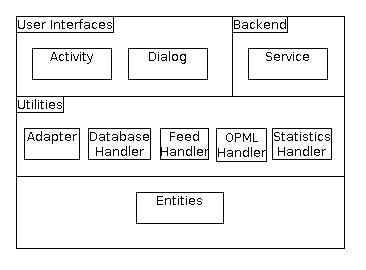
\includegraphics[width=0.8\textwidth]{./images/ApplicationLayers.png}
\caption{Layers of the Application Architecture}
\label{fig:app_layers}
\end{figure}
To allow the user to input information such as category names or feed links \textit{Dialogs} are used, based on the \textit{Android} class \textit{DialogFragment}. The complete architecture of the application is shown in figure~\ref{fig:app_layers} divided into different layers. The two top layers are the actual application, \textit{User Interfaces} and \textit{Backend}, and utilizes the middle layer \textit{Utilities}. These give fully access and control over the lower layer containing the \textit{Entities}. In the current architecture all the \textit{Utilities} are connected to all the types of \textit{Entities}. 
\begin{figure}[hbt]
\centering
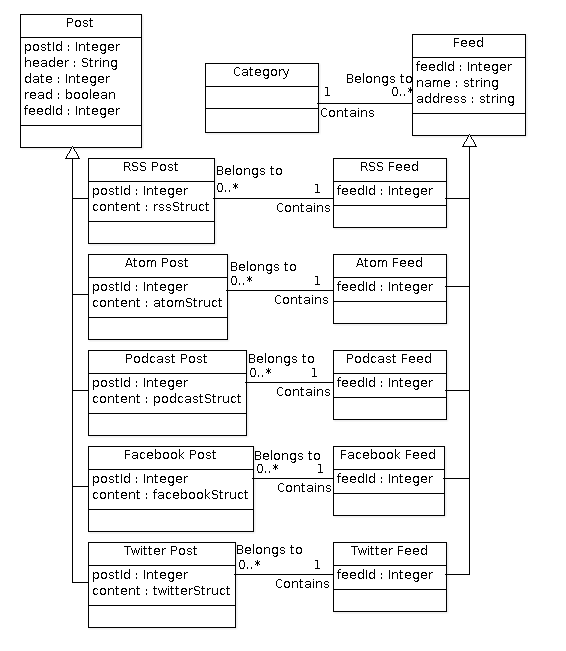
\includegraphics[width=0.8\textwidth]{./images/EntityClassDiagram.png}
\caption{Entity Class Diagram of the Product}
\label{fig:entity}
\end{figure}
The \textit{Entities} of the application are \textit{Category}, \textit{Feed} and \textit{Post} and are shown in figure~\ref{fig:entity}. Here all sub-entities are included and their relationship to each other.

\newpage
\subsection{System Features}
\label{sec:system_features}
In this section are all the included system features examined and described with the help of their respective class diagram.


\subsubsection{Share Post}
\begin{figure}[hbt]
\centering
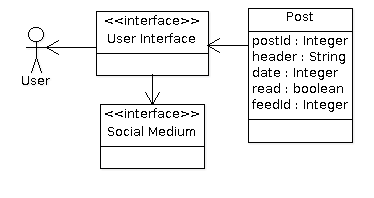
\includegraphics[width=0.45\textwidth]
{./images/SharePost.png}
\caption{Class Diagram of system feature Share Post}
\label{fig:share}
\end{figure}
The ability to share a post requires two things, a post to share and a target to share it to. The relationship required to perform this feature is visualized in figure~\ref{fig:share}. Here the user has the ability through the user interface to share a post to a social medium of its choice. The social medium is accessed through an interface to its API. \\
\begin{tabular}{l l}
\begin{minipage}{0.5\textwidth}
\begin{enumerate}
  \item Access the post view, shown in figure~\ref{fig:share_screen}.
  \item Display all actions by pressing the \textit{Menu} button on the device.
  \item Press \textit{Share Post}.
  \item In the displayed dialog enter the required credentials to be able to share the post the chosen medium.
\end{enumerate}
\end{minipage}
&
\begin{minipage}{0.5\textwidth}
  \centering
  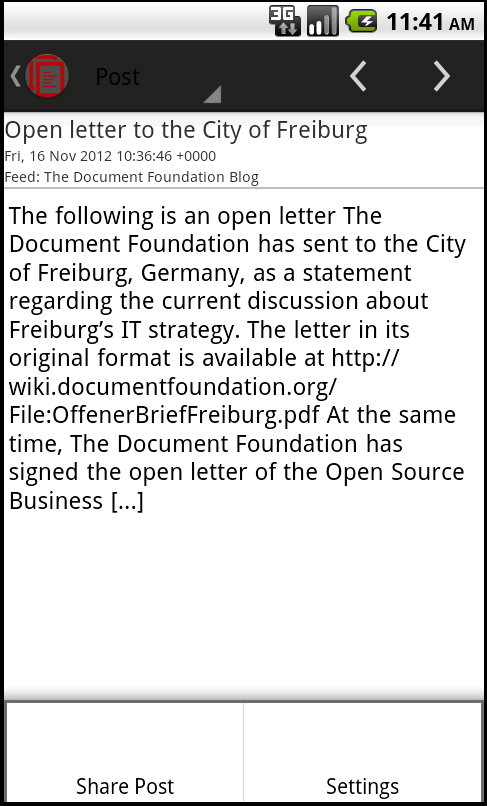
\includegraphics[width=0.8\textwidth]{./images/PostOptions.png}
  \captionof{figure}{Screenshot of the post view}
  \label{fig:share_screen}
\end{minipage}
\end{tabular}


\newpage
\subsubsection{Count Un-read Post(s)}
\begin{figure}[hbt]
\centering
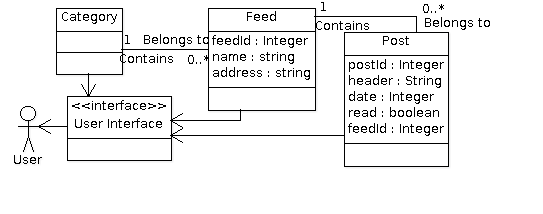
\includegraphics[width=0.6\textwidth]
{./images/CountUnreadPosts.png}
\caption{Class Diagram of system feature Count Un-read Post(s)}
\label{fig:count}
\end{figure}
To count un-read post(s) access to not only the posts but also the feeds and the feed list are required so that posts of all feeds are accounted for. The relationship required to perform this feature is visualized in figure~\ref{fig:count}. Here the user accesses the number of un-read post(s) through the user interface which in turn is connected to all the required classes to determine the total un-read post(s) count. \\
\begin{tabular}{l l}
\begin{minipage}{0.5\textwidth}
\begin{enumerate}
  \item Access the feed view, shown in figure~\ref{fig:count_screen}.
  \item Unread posts are shown as bold in the list, while read posts are not bold.
\end{enumerate}
\textit{The total amount of unread posts can be accessed internally through a database query, and implemented to be shown where it fits.}
\end{minipage}
&
\begin{minipage}{0.5\textwidth}
  \centering
  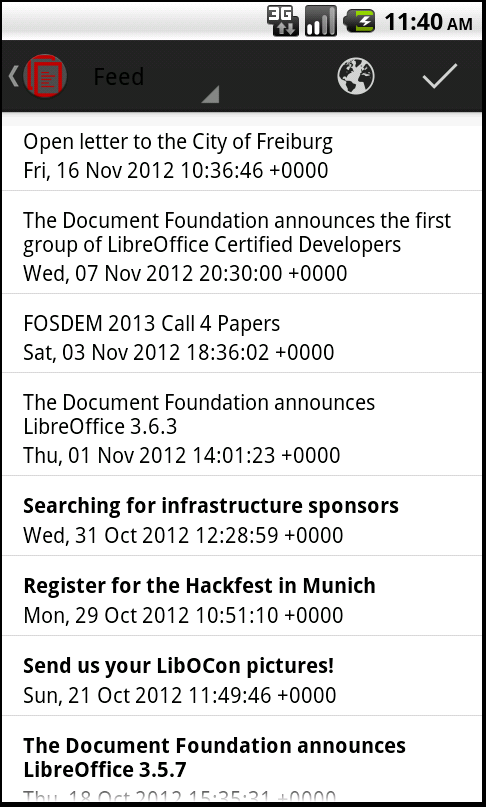
\includegraphics[width=0.8\textwidth]{./images/ViewReadAndUnreadPosts.png}
  \captionof{figure}{Screenshot of the feed view}
  \label{fig:count_screen}
\end{minipage}
\end{tabular}


\newpage
\subsubsection{Read Post(s)}
\begin{figure}[hbt]
\centering
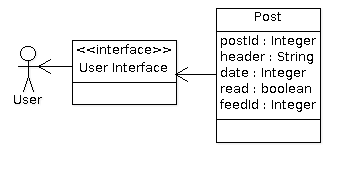
\includegraphics[width=0.45\textwidth]
{./images/ReadPosts.png}
\caption{Class Diagram of system feature Read Post(s)}
\label{fig:read}
\end{figure}
For users to access and read post(s) an user interface is required that is connected to the actual post(s). The relationship required to perform this feature is visualized in figure~\ref{fig:read}. The user interface will determines which post(s) based on previous state, e.g. which post the user has selected to read coming from a previous view. \\
\begin{tabular}{l l}
\begin{minipage}{0.5\textwidth}
\begin{enumerate}
  \item Access the post view, shown in figure~\ref{fig:post_screen}.
  \item Be notified by the interface that the post has been marked as read.
  \item Read title, publication date and source feed in the header.
  \item Read the description, that may include pictures, below the header.
  \item To access the actually post through a web browser click the title in the header.
\end{enumerate}
\end{minipage}
&
\begin{minipage}{0.5\textwidth}
  \centering
  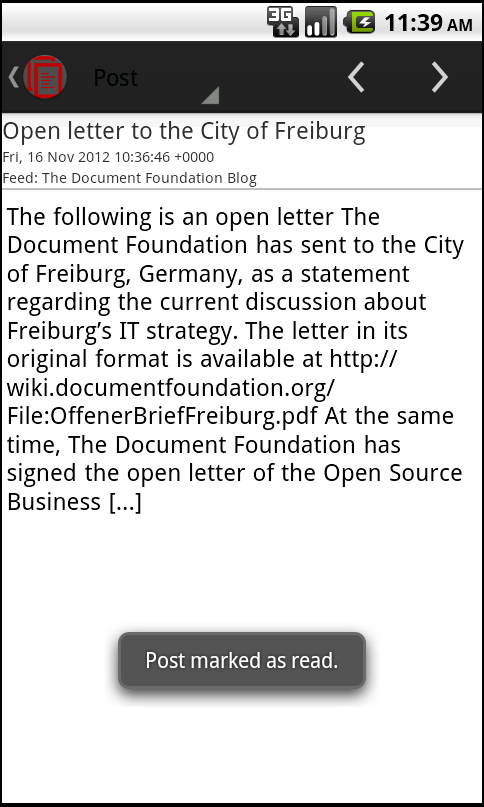
\includegraphics[width=0.8\textwidth]{./images/MarkPostRead.png}
  \captionof{figure}{Screenshot of the post view}
  \label{fig:post_screen}
\end{minipage}
\end{tabular}


\newpage
\subsubsection{View Feed(s)}
\begin{figure}[hbt]
\centering
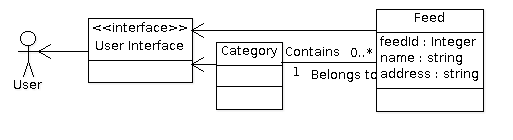
\includegraphics[width=0.6\textwidth]
{./images/ViewFeeds.png}
\caption{Class Diagram of system feature View Feed(s)}
\label{fig:view}
\end{figure}
Users access and view feed(s) through an user interface that is connected to the feed(s). The relationship required to perform this feature is visualized in figure~\ref{fig:view}. The user interface determines which feed(s) based on previous state, e.g. which category of feeds the user has selected to view coming from a previous view. \\
\begin{tabular}{l l}
\begin{minipage}{0.5\textwidth}
\begin{enumerate}
  \item Access the feed view, shown in figure~\ref{fig:feed_screen}.
  \item The 30 latest posts are shown in a scrollable list.
  \item Press a post to access the post view for that specific post.
\end{enumerate}
\end{minipage}
&
\begin{minipage}{0.5\textwidth}
  \centering
  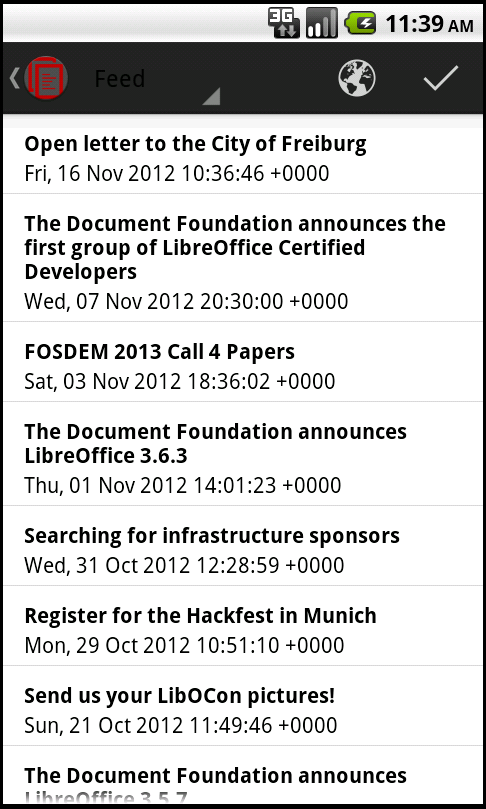
\includegraphics[width=0.8\textwidth]{./images/ViewPosts.png}
  \captionof{figure}{Screenshot of the feed view}
  \label{fig:feed_screen}
\end{minipage}
\end{tabular}


\newpage
\subsubsection{View Statistics}
\begin{figure}[hbt]
\centering
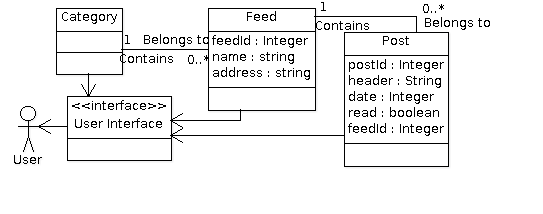
\includegraphics[width=0.6\textwidth]
{./images/CountUnreadPosts.png}
\caption{Class Diagram of system feature View Statistics}
\label{fig:statistics}
\end{figure}
To view statistics access to not only the posts but also the feeds and the feed list are required so that all statistics on all levels are collected. The relationship required to perform this feature is visualized in figure~\ref{fig:count}. Here the user accesses the statistics through the user interface which in turn is connected to all the required classes to collect all interesting data. \\
\begin{tabular}{l l}
\begin{minipage}{0.5\textwidth}
\begin{enumerate}
  \item Access any view of feed level or higher, shown in figure~\ref{fig:feed_opt_screen}.
  \item Display all actions by pressing the \textit{Menu} button on the device.
  \item Press \textit{Statistics}.
  \item In the displayed dialog statistics are shown for the current level.
\end{enumerate}
\end{minipage}
&
\begin{minipage}{0.5\textwidth}
  \centering
  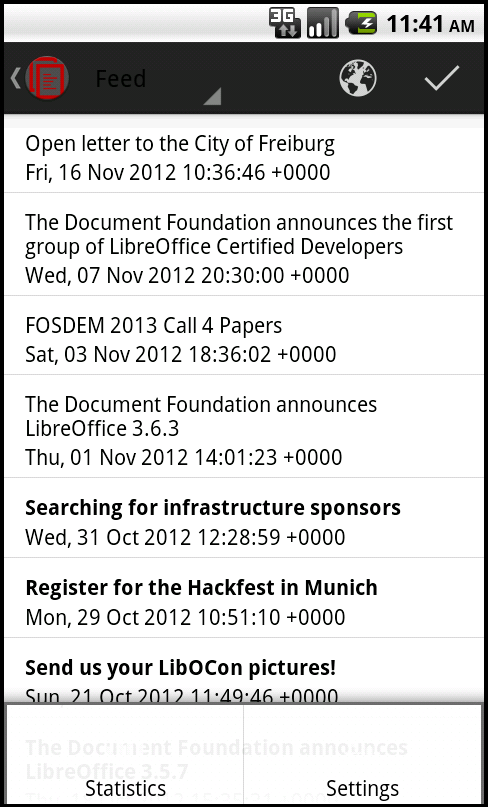
\includegraphics[width=0.8\textwidth]{./images/FeedOptions.png}
  \captionof{figure}{Screenshot of the feed view}
  \label{fig:feed_opt_screen}
\end{minipage}
\end{tabular}


\newpage
\subsubsection{Import/Export Feed(s)}
\begin{figure}[hbt]
\centering
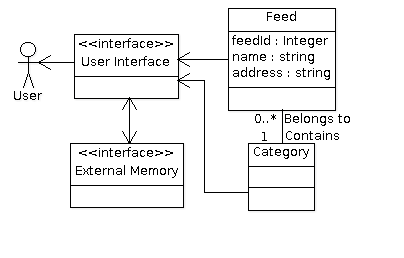
\includegraphics[width=0.5\textwidth]
{./images/ImportExportFeeds.png}
\caption{Class Diagram of system feature Import/Export Feed(s)}
\label{fig:import}
\end{figure}
By an interface to a storage area, external memory in the case of Android, the user has the possible to either import a set of feed(s) or export. The relationship required to perform this feature is visualized in figure~\ref{fig:import}. Both actions are triggered through the user interface. For importing the user chooses a file on external memory, with a standardized file format for feed lists, and the product performs a mass add of the feeds in the file. An export action from the user will create a feed list file, with the same standardized file format as mentioned earlier. \\
\begin{tabular}{l l}
\begin{minipage}{0.5\textwidth}
\begin{enumerate}
  \item Access the main view, shown in figure~\ref{fig:import_screen}.
  \item Display all actions by pressing the \textit{Menu} button on the device.
  \item Press \textit{Import/Export Feeds}.
  \item In the displayed dialog chose if you want to import or export feeds.
  \item In the following dialog chose either which file to import or what file name to export to.
\end{enumerate}
\end{minipage}
&
\begin{minipage}{0.5\textwidth}
  \centering
  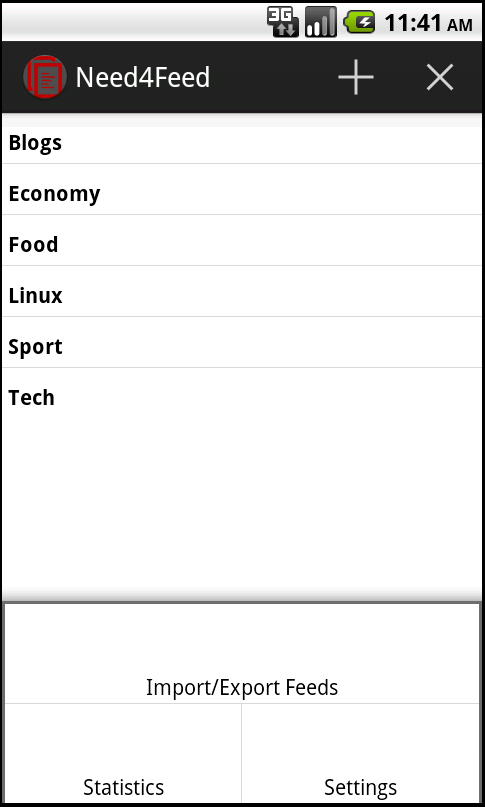
\includegraphics[width=0.8\textwidth]{./images/ImportExport.png}
  \captionof{figure}{Screenshot of the main view}
  \label{fig:import_screen}
\end{minipage}
\end{tabular}


\newpage
\subsubsection{Find Similar Feed(s)}
\begin{figure}[hbt]
\centering
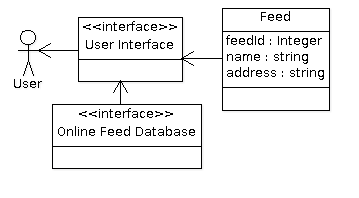
\includegraphics[width=0.5\textwidth]
{./images/FindSimilarFeeds.png}
\caption{Class Diagram of system feature Find Similar Feed(s)}
\label{fig:find}
\end{figure}
When a user has a feed and wants to find similar feeds he can through the user interface trigger a search. The relationship required to perform this feature is visualized in figure~\ref{fig:find}. The search will look in online feed databases, through their web-based API's, based on data from the feed in form of name and address. \\
\begin{tabular}{l l}
\begin{minipage}{0.5\textwidth}
\begin{enumerate}
  \item Access the feed view, shown in figure~\ref{fig:find_screen}.
  \item Press \textit{Find Similar Feeds}, shown as the first icon in the action bar visualized as a globe.
  \item In the displayed dialog chose which similar feed you like to add.
\end{enumerate}
\end{minipage}
&
\begin{minipage}{0.5\textwidth}
  \centering
  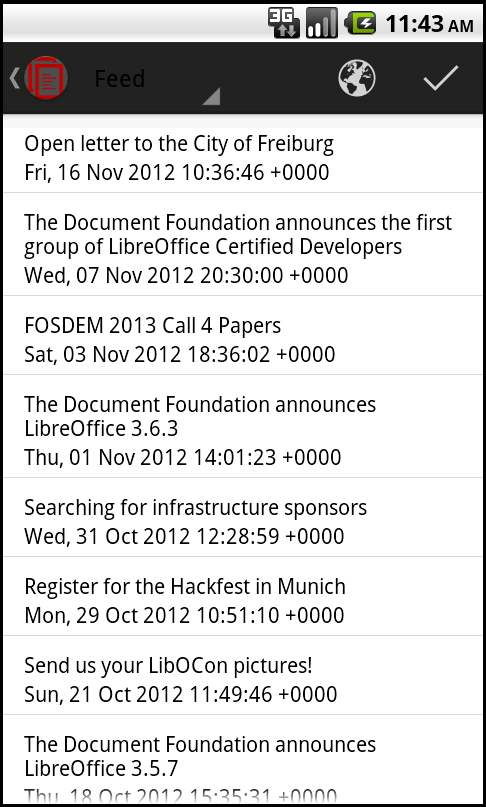
\includegraphics[width=0.8\textwidth]{./images/ViewReadPosts.png}
  \captionof{figure}{Screenshot of the feed view}
  \label{fig:find_screen}
\end{minipage}
\end{tabular}


\newpage
\subsubsection{Manage Feed(s)}
\begin{figure}[hbt]
\centering
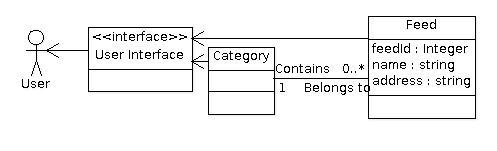
\includegraphics[width=0.5\textwidth]
{./images/ManageFeeds.png}
\caption{Class Diagram of system feature Manage Feed(s)}
\label{fig:manage}
\end{figure}
For a user, or administrator to be exact, to manage feeds he has to do so through the user interface in which there are options and functions to perform all required sub-features. The relationship required to perform this feature is visualized in figure~\ref{fig:manage}. In this case the user interface is directly connected to the feed list and feed(s). \\
\begin{tabular}{l l}
\begin{minipage}{0.5\textwidth}
\begin{enumerate}
  \item Access the main view, shown in figure~\ref{fig:add_category_screen}.
  \item Press \textit{Add Category}, shown as the first icon in the action bar visualized as a plus sign.
  \item In the displayed dialog chose a name for the category.
\end{enumerate}
\end{minipage}
&
\begin{minipage}{0.5\textwidth}
  \centering
  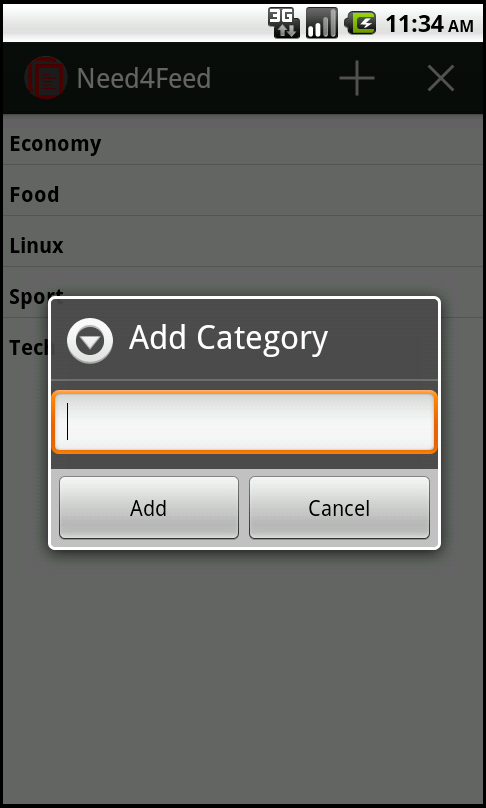
\includegraphics[width=0.8\textwidth]{./images/AddCategory.png}
  \captionof{figure}{Screenshot of the add category dialog}
  \label{fig:add_category_screen}
\end{minipage}
\end{tabular} \\
\begin{tabular}{l l}
\begin{minipage}{0.5\textwidth}
\begin{enumerate}
  \item Access the category view, shown in figure~\ref{fig:add_feed_screen}.
  \item Press \textit{Add Feed}, shown as the first icon in the action bar visualized as a plus sign.
  \item In the displayed dialog enter the url address to the feed to be added.
\end{enumerate}
\end{minipage}
&
\begin{minipage}{0.5\textwidth}
  \centering
  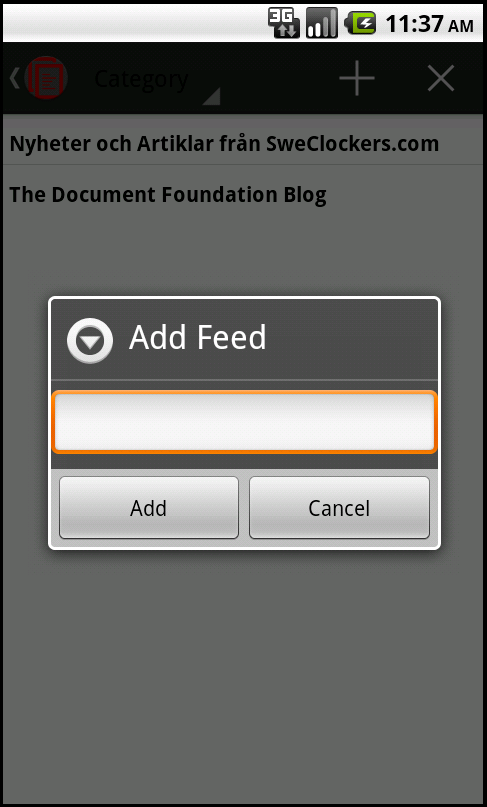
\includegraphics[width=0.8\textwidth]{./images/AddFeed.png}
  \captionof{figure}{Screenshot of the add feed dialog}
  \label{fig:add_feed_screen}
\end{minipage}
\end{tabular}


\newpage
\subsection{Directory Organization}
\label{sec:directory_organization}
The structure of the project is the default structure of an \textit{Eclipse} project for \textit{Android} using the \textit{ADT}. The source file are located in \textit{/src/} with a substructure based on the \textit{Java} packages they are located in, something that is mandatory for \textit{Android projects}. The used packages has to be completely unique to latter on be accepted into \textit{Google Play}, the online application market for \textit{Android}. 
\begin{table}[hbt]
\begin{center}
    \begin{tabular}{ | l | l |}
    \hline
    \textbf{Directory} & \textbf{File name}\\ \hline
    /src/bit/app/need4feed/ & MainApplication.java\\ \hline
    /src/bit/app/need4feed/ & MainActivity.java\\ \hline
    /src/bit/app/need4feed/ & CategoryActivity.java\\ \hline
    /src/bit/app/need4feed/ & FeedActivity.java\\ \hline
    /src/bit/app/need4feed/ & PostActivity.java\\ \hline
    /src/bit/app/need4feed/ & RssService.java\\ \hline
    /src/bit/app/need4feed/ & AddCategoryDialog.java\\ \hline
    /src/bit/app/need4feed/ & RemoveCategoryDialog.java\\ \hline
    /src/bit/app/need4feed/ & AddFeedDialog.java\\ \hline
    /src/bit/app/need4feed/ & RemoveFeedDialog.java\\ \hline
    /src/bit/app/need4feed/util/ & DatabaseHandler.java\\ \hline
    /src/bit/app/need4feed/util/ & RssHandler.java\\ \hline
    /src/bit/app/need4feed/util/ & OpmlHandler.java\\ \hline
    /src/bit/app/need4feed/type/ & Category.java\\ \hline
    /src/bit/app/need4feed/type/ & CategoryAdapter.java\\ \hline
    /src/bit/app/need4feed/type/ & Feed.java\\ \hline
    /src/bit/app/need4feed/type/ & FeedAdapter.java\\ \hline
    /src/bit/app/need4feed/type/ & Post.java\\ \hline
    /src/bit/app/need4feed/type/ & PostAdapter.java\\ \hline
    \end{tabular}
    \caption{Directory Organization of Android Source Files}\label{tab:directory_organization_source}
\end{center}
\end{table}
Beyond source files, seen in table~\ref{tab:directory_organization_source}, an \textit{Android} project also contains \textit{XML} files used for layouts for activities, dialogs and menus. \textit{XML} files are also used for strings used graphically throughout the program. All of these \textit{XML} files are located under \textit{/res/layout/}, \textit{/res/menu/} and \textit{/res/strings/}. In addition to \textit{XML} files \textit{/res/} also includes image files used for icons and symbols, these are located in their respective \textit{/res/drawable/} directory. All files under \textit{/res/} are resources that are used dynamically during runtime, this design enables \textit{Android} to change the its look while running based on feature such as size of phone or as simple as the current orientation of the screen.
\begin{table}[hbt]
\begin{center}
    \begin{tabular}{ | l | l |}
    \hline
    \textbf{Directory} & \textbf{File name}\\ \hline
	/res/layout/ & *.xml\\ \hline
	/res/menu/ & *.xml\\ \hline
	/res/strings/ & *.xml\\ \hline
    /res/drawable-hdpi/ & *.png\\ \hline
    /res/drawable-ldpi/ & *.png\\ \hline
    /res/drawable-mdpi/ & *.png\\ \hline
    /res/drawable-xhdpi/ & *.png\\ \hline
    \end{tabular}
    \caption{Directory Organization of Android Resource Files}\label{tab:directory_organization_resource}
\end{center}
\end{table}
The directory organization of the resource files are shown in table~\ref{tab:directory_organization_resource}.


\subsection{Class Description}
\label{sec:class_description}

\subsubsection{MainApplication}
\textit{MainApplication} belongs to the \textit{Backend} layer of the architecture but is however not a \textit{Service}. This class extends the \textit{Android} class \textit{Application} and has the purpose to create a structure with a different life-cycle than of the activities, that can pause or terminate at any point and later on be re-created if returned to. With this feature, of being non-terminated until the application is terminated, \textit{MainApplication} gives the functionality to hold truly global variables and instances accessible to all activities through the \textit{Android} virtual machine.
\begin{description}
  \item[Location:] \textit{/src/bit/app/need4feed/MainApplication.java} \hfill
  \item[Class Components:] \hfill
     \begin{itemize}
        \item databaseHandler: DatabaseHandler
        \item getDatabaseHandler(): DatabaseHandler
     \end{itemize}
\end{description}


\subsubsection{MainActivity}
\textit{MainActivity} is the main user interface and the entry screen of the application, it extends \textit{Activity} and belongs to the \textit{User Interfaces} layer of the architecture. The purpose of the class is to create the first view, holding a list of all categories. It also takes the user to the next view when a category has been clicked. \textit{MainActivity} gives the functionality, beyond displaying categories and managing the transition to \textit{CategoryActivity}, to add and remove categories.
\begin{description}
  \item[Location:] \textit{/src/bit/app/need4feed/MainActivity.java} \hfill
  \item[Class Components:] \hfill
     \begin{itemize}
        \item actionBar: ActionBar
        \item categoryListView: ListView
        \item categoryAdapter: CategoryAdapter
        \item databaseHandler: DatabaseHandler
        \item onFinishAddCategoryDialog(): void
        \item onFinishRemoveCategoryDialog(): void
     \end{itemize}
\end{description}


\subsubsection{CategoryActivity}
\textit{CategoryActivity} is the second activity the user gets in contact with, it extends \textit{Activity} and belongs to the \textit{User Interfaces} layer of the architecture. The purpose of the class is to create a list view of feeds for a certain category, thereby the name \textit{CategoryActivity}. It gives the functionality, except to list all feeds of a category, to take the user to a certain feed if clicked on as well as add and remove feeds to that specific category.
\begin{description}
  \item[Location:] \textit{/src/bit/app/need4feed/CategoryActivity.java} \hfill
  \item[Class Components:] \hfill
     \begin{itemize}
        \item actionBar: ActionBar
        \item feedListView: ListView
        \item feedAdapter: FeedAdapter
        \item databaseHandler: DatabaseHandler
        \item categoryId: long
        \item onFinishAddFeedDialog(): void
        \item onFinishRemoveFeedDialog(): void
     \end{itemize}
\end{description}


\subsubsection{FeedActivity}
\textit{FeedActivity} is the third activity the user gets in contact with, it extends \textit{Activity} and belongs to the \textit{User Interfaces} layer of the architecture. The purpose of the class is to create a list view of posts for a certain feed, thereby the name \textit{FeedActivity}. It gives the functionality, except to list all posts of a feed, to take the user to a certain post if clicked on.
\begin{description}
  \item[Location:] \textit{/src/bit/app/need4feed/FeedActivity.java} \hfill
  \item[Class Components:] \hfill
     \begin{itemize}
        \item actionBar: ActionBar
        \item postListView: ListView
        \item postAdapter: PostAdapter
        \item databaseHandler: DatabaseHandler
        \item feedId: long
     \end{itemize}
\end{description}


\subsubsection{PostActivity}
\textit{PostActivity} is the fourth, and last, activity the user gets in contact with, it extends \textit{Activity} and belongs to the \textit{User Interfaces} layer of the architecture. The purpose of the class is to display a specific post and its content, thereby the name \textit{PostActivity}. It gives the functionality, except to display a post, to take the user to the web page of the post through a click on the post heading.
\begin{description}
  \item[Location:] \textit{/src/bit/app/need4feed/PostActivity.java} \hfill
  \item[Class Components:] \hfill
     \begin{itemize}
        \item actionBar: ActionBar
        \item titleTextView: TextView
        \item feedTextView: TextView
        \item contentWebView: WebView
        \item sourceFeed: Feed
        \item displayedPost: Post
        \item databaseHandler: DatabaseHandler
        \item postId: long
     \end{itemize}
\end{description}

	
\subsubsection{RssService}
\textit{RssService} extends \textit{Intent Service} and belongs to the \textit{Backend} layer of the architecture. The purpose of this class is to serve as a background task, periodically fetching the latest posts. Its functionality is built up out off two parts; database access to both fetch all existing feeds and then store all new posts as well as access the actual \textit{RSS} feeds.
\begin{description}
  \item[Location:] \textit{/src/bit/app/need4feed/RssService.java} \hfill
  \item[Class Components:] \hfill
     \begin{itemize}
        \item databaseHandler: DatabaseHandler
        \item rssHandler: RssHandler
     \end{itemize}
\end{description}


\subsubsection{AddCategoryDialog}
\textit{AddCategoryDialog} is a \textit{Dialog} and belongs to the \textit{User Interface} layer of the architecture. The class extends \textit{DialogFragment} to enable all required \textit{Dialog} functionality. The purpose of this class is to create the user interface that enables the user to input a category name and create a category. Furthermore the functionality includes adding the new category to the database and signal the associated \textit{Activity} through \textit{addCategoryDialogListener} which is connected to \textit{MainActivity}.
\begin{description}
  \item[Location:] \textit{/src/bit/app/need4feed/AddCategoryDialog.java} \hfill
  \item[Class Components:] \hfill
     \begin{itemize}
        \item databaseHandler: DatabaseHandler
        \item addCategoryDialogListener: AddCategoryDialogListener
     \end{itemize}
\end{description}


\subsubsection{RemoveCategoryDialog}
\textit{RemoveCategoryDialog} is a \textit{Dialog} and belongs to the \textit{User Interface} layer of the architecture. The class extends \textit{DialogFragment} to enable all required \textit{Dialog} functionality. The purpose of this class is to create the user interface that enables the user to input which category to remove. Furthermore the functionality includes removing the specific category from the database and signal the associated \textit{Activity} through \textit{removeCategoryDialogListener} which is connected to \textit{MainActivity}.
\begin{description}
  \item[Location:] \textit{/src/bit/app/need4feed/RemoveCategoryDialog.java} \hfill
  \item[Class Components:] \hfill
     \begin{itemize}
        \item databaseHandler: DatabaseHandler
        \item removeCategoryDialogListener: RemoveCategoryDialogListener
     \end{itemize}
\end{description}


\subsubsection{AddFeedDialog}
\textit{AddFeedDialog} is a \textit{Dialog} and belongs to the \textit{User Interface} layer of the architecture. The class extends \textit{DialogFragment} to enable all required \textit{Dialog} functionality. The purpose of this class is to create the user interface that enables the user to input a feed link and create a feed. Furthermore the functionality includes adding the new feed to the database, fetch the latest posts for it, and signal the associated \textit{Activity} through \textit{addFeedDialogListener} which is connected to \textit{CategoryActivity}.
\begin{description}
  \item[Location:] \textit{/src/bit/app/need4feed/AddFeedDialog.java} \hfill
  \item[Class Components:] \hfill
     \begin{itemize}
        \item databaseHandler: DatabaseHandler
        \item addFeedDialogListener: AddFeedDialogListener
     \end{itemize}
\end{description}


\subsubsection{RemoveFeedDialog}
\textit{RemoveFeedDialog} is a \textit{Dialog} and belongs to the \textit{User Interface} layer of the architecture. The class extends \textit{DialogFragment} to enable all required \textit{Dialog} functionality. The purpose of this class is to create the user interface that enables the user to input which feed to remove. Furthermore the functionality includes removing the specific feed from the database and signal the associated \textit{Activity} through \textit{removeFeedDialogListener} which is connected to \textit{CategoryActivity}.
\begin{description}
  \item[Location:] \textit{/src/bit/app/need4feed/RemoveFeedDialog.java} \hfill
  \item[Class Components:] \hfill
     \begin{itemize}
        \item databaseHandler: DatabaseHandler
        \item removeFeedDialogListener: RemoveFeedDialogListener
     \end{itemize}
\end{description}


\subsubsection{DatabaseHandler}
\textit{DatabaseHandler} is part of the \textit{Utilities} layer of the architecture and works as a \textit{Singleton} class as it is only initiated within the \textit{MainApplication}. To enable \textit{SQLite} functionality it extends \textit{SQLiteOpenHelper}. The purpose of this class is to handle all queries to and from the database containing all entities. 
\begin{description}
  \item[Location:] \textit{/src/bit/app/need4feed/util/DatabaseHandler.java} \hfill
  \item[Class Components:] \hfill
     \begin{itemize}
        \item db: SQLiteDatabase
		\item addCategory(Category): void 
		\item addFeed(Feed): void
		\item addPost(Post): void
		\item updateCategory(Category): void
		\item updateFeed(Feed): void
		\item updatePost(Post): void
		\item deleteCategory(long): void
		\item deleteFeed(long): void
		\item deletePostOfFeed(long): void
		\item deletePost(long): void
		\item getCategories(): List\textless Category\textgreater
		\item getCategoryNames(): String[]
		\item getAllFeeds(): List\textless Feed\textgreater
		\item getFeeds(long): List\textless Feed\textgreater
		\item getFeedNames(long): String[]
		\item getFeed(long): Feed
		\item getPosts(long): List\textless Post\textgreater
		\item getPost(long): Post
		\item getPostCount(long) int
     \end{itemize}
\end{description}


\subsubsection{RssHandler}
\textit{RssHandler} is part of the \textit{Utilities} layer of the architecture and extends \textit{DefaultHandler} to be able to process \textit{XML} files. The class imports \textit{SAXParser} to help parse tags. The functionality of \textit{RssHandler} is to access the \textit{Internet} and fetch \textit{RSS} \textit{XML} files and process them, either to fetch information about a feed or its posts. The class then stores the information in the database.
\begin{description}
  \item[Location:] \textit{/src/bit/app/need4feed/util/RssHandler.java} \hfill
  \item[Class Components:] \hfill
     \begin{itemize}
        \item db: DatabaseHandler
        \item currentFeed: Feed
        \item currentPost: Post
        \item postList: List\textless Post\textgreater
		\item verifyFeed(String): String 
		\item getFeed(String): Feed
		\item getAllLatestPosts(): void
		\item getLatestPosts(Feed): void
     \end{itemize}
\end{description}


\subsubsection{OpmlHandler}
\textit{OpmlHandler} is part of the \textit{Utilities} layer of the architecture and extends \textit{DefaultHandler} to be able to process \textit{XML} files. The class imports \textit{SAXParser} to help parse tags. The functionality of \textit{OpmlHandler} is to process feed lists written in \textit{OPML} file format, that expends \textit{XML}. It enables both import and export of feed lists.
\begin{description}
  \item[Location:] \textit{/src/bit/app/need4feed/util/OpmlHandler.java} \hfill
  \item[Class Components:] \hfill
     \begin{itemize}
        \item db: DatabaseHandler
		\item ImportFeeds( File file ): void
		\item ExportFeeds( void ): File
     \end{itemize}
\end{description}


\subsubsection{Category}
\textit{Category}, the entity class, of the \textit{Entities} layer of the architecture. The purpose of this class is to symbolize an entity and manage its variables. Also included is a \textit{compareTo} method to deal with sorting of the entity, for categories the sorting is done alphabetically.
\begin{description}
  \item[Location:] \textit{/src/bit/app/need4feed/type/Category.java} \hfill
  \item[Class Components:] \hfill
     \begin{itemize}
        \item id: long
        \item name: String
		\item getId(): long 
		\item setId(long): void
		\item getName(): String 
		\item setName(String): void
		\item compareTo(Category): int
     \end{itemize}
\end{description}


\subsubsection{CategoryAdapter}
\textit{CategoryAdapter} is utility tight connected to its type, \textit{Category}, and is part of the \textit{Utilities} layer of the architecture. Its purpose is to handle lists of categories and present them in \textit{ListViews}.
\begin{description}
  \item[Location:] \textit{/src/bit/app/need4feed/type/CategoryAdapter.java} \hfill
  \item[Class Components:] \hfill
     \begin{itemize}
        \item categoryList: List\textless Category\textgreater
        \item holder: ViewHolder
		\item setCategoryList(List\textless Category\textgreater): void 
     \end{itemize}
\end{description}


\subsubsection{Feed}
\textit{Feed}, the entity class, of the \textit{Entities} layer of the architecture. The purpose of this class is to symbolize an entity and manage its variables. Also included is a \textit{compareTo} method to deal with sorting of the entity, for feeds the sorting is done alphabetically.
\begin{description}
  \item[Location:] \textit{/src/bit/app/need4feed/type/Feed.java} \hfill
  \item[Class Components:] \hfill
     \begin{itemize}
        \item id: long
        \item categoryId: long
        \item title: String
        \item link: String
        \item feedLink: String
        \item description: String
		\item getId(): long 
		\item setId(long): void
		\item getCategoryId(): long 
		\item setCategoryId(long): void
		\item getTitle(): String 
		\item setTitle(String): void
		\item getLink(): String 
		\item setLink(String): void
		\item getFeedLink(): String 
		\item setFeedLink(String): void
		\item getDescription(): String 
		\item setDescription(String): void
		\item compareTo(Feed): int
     \end{itemize}
\end{description}


\subsubsection{FeedAdapter}
\textit{FeedAdapter} is utility tight connected to its type, \textit{Feed}, and is part of the \textit{Utilities} layer of the architecture. Its purpose is to handle lists of categories and present them in \textit{ListViews}.
\begin{description}
  \item[Location:] \textit{/src/bit/app/need4feed/type/FeedAdapter.java} \hfill
  \item[Class Components:] \hfill
     \begin{itemize}
        \item feedList: List\textless Feed\textgreater
        \item holder: ViewHolder
		\item setFeedList(List\textless Feed\textgreater): void 
     \end{itemize}
\end{description}


\subsubsection{Post}
\textit{Post}, the entity class, of the \textit{Entities} layer of the architecture. The purpose of this class is to symbolize an entity and manage its variables. Also included is a \textit{compareTo} method to deal with sorting of the entity, for posts the sorting is done based on the date which is stored in \textit{pubDate}.
\begin{description}
  \item[Location:] \textit{/src/bit/app/need4feed/type/Post.java} \hfill
  \item[Class Components:] \hfill
     \begin{itemize}
        \item id: long
        \item feedId: long
        \item title: String
        \item link: String
        \item description: String
        \item pubDate: String
        \item thumbnail: String
		\item getId(): long 
		\item setId(long): void
		\item getFeedId(): long 
		\item setFeedId(long): void
		\item getTitle(): String 
		\item setTitle(String): void
		\item getLink(): String 
		\item setLink(String): void
		\item getDescription(): String 
		\item setDescription(String): void
		\item getPubDate(): String 
		\item setPubDate(String): void
		\item getThumbnail(): String 
		\item setThumbnail(String): void
		\item compareTo(Post): int
     \end{itemize}
\end{description}


\subsubsection{PostAdapter}
\textit{PostAdapter} is utility tight connected to its type, \textit{Post}, and is part of the \textit{Utilities} layer of the architecture. Its purpose is to handle lists of categories and present them in \textit{ListViews}.
\begin{description}
  \item[Location:] \textit{/src/bit/app/need4feed/type/PostAdapter.java} \hfill
  \item[Class Components:] \hfill
     \begin{itemize}
        \item postList: List\textless Post\textgreater
        \item holder: ViewHolder
		\item setPostList(List\textless Post\textgreater): void 
     \end{itemize}
\end{description}




% that's all folks
\end{document}